\documentclass[11pt,a4paper]{report}
\usepackage[utf8]{inputenc}
\usepackage{amsmath}
\usepackage{graphicx}
\usepackage{gensymb}
\usepackage{tikz}
\usetikzlibrary{positioning}
\usepackage{geometry}
\geometry{
    left=2cm,
    right=0.64cm,
    top=0.64cm,
    bottom=2cm
}
\usepackage{multicol}
\setlength{\columnsep}{1cm}
\graphicspath{ {images/} }

\begin{document}

\chapter{Semester 2 Examination 2014-2015\\CZ4034 Information Retrieval}

\begin{multicols*}{2}

\section{Question 1}
\noindent \textbf{Question 1a} Explain the following concepts with examples

\noindent \textbf{(i)} Posting list: It is a list of document IDs that contain a specific dictionary term, and is used in inverted index. The posting list needs to be a variable size list so that new documents can be added easily to the list. 

\begin{center}
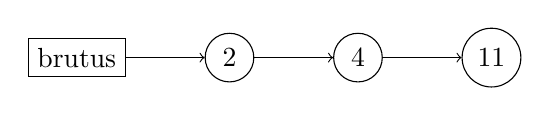
\begin{tikzpicture}[
squarenode/.style={rectangle, draw=black, thin},
roundnode/.style={circle, draw=black, thin},
]
%Nodes
\node[squarenode](brutus){brutus};
\node[roundnode](2)[right=of brutus]{2};
\node[roundnode](4)[right=of 2]{4};
\node[roundnode](11)[right=of 4]{11};

\draw[->](brutus.east) -- (2.west);
\draw[->](2.east) -- (4.west);
\draw[->](4.east) -- (11.west);
\end{tikzpicture}
\end{center}

\noindent \textbf{(ii)} Biword index: We use two consecutive words as dictionary pharases, instead of using unigram which treat each words as dictionary terms. For example, if we have the following sentence:
\begin{center}
\verb|I am a boy|
\end{center}
\noindent Then our dictionary phrases are: \verb|I am|, \verb|am a|, \verb|a boy|. \\

\noindent \textbf{(iii)} Stemming: Reduce terms to their “roots”, by crude chopping. For example:
\begin{itemize}
    \item automates automatic automation $\rightarrow$ automat
    \item democrats $\rightarrow$ democrat (noun)
    \item democratized $\rightarrow$ democratize (verb)
\end{itemize} 

\noindent \textbf{Question 1b} Given the entries of the permuterm index for the following terms: \verb|one|, \verb|two|, \verb|three|.

\noindent Answer: \verb|one$|, \verb|ne$o|, \verb|e$on|, \verb|$one|, \verb|two$|, \verb|wo$t|, \verb|o$tw|, \verb|$two|, \verb|three$|, \verb|hree$t|, \verb|ree$th|, \verb|ee$thr|, \verb|e$thre|, \verb|$three|\\

\noindent \textbf{Question 1c} Calculate the edit distance between \verb|work| and \verb|walk| by using Levenshtein distance algorithm

\begin{center}
\begin{tabular}{ | l | l  l  l  l  l |} 
    \hline
      &   & w & o & r & k \\
    \hline
      & 0 & 1 & 2 & 3 & 4 \\
    w & 1 & 0 & 1 & 2 & 3 \\
    a & 2 & 1 & 1 & 2 & 3 \\
    l & 3 & 2 & 2 & 2 & 3 \\
    k & 4 & 3 & 3 & 3 & \textbf{2} \\
    \hline
\end{tabular}
\end{center}

\noindent \textbf{Question 1d} Assume that you use the combination of three compression techniques of dictionary-as-strings, block($k=2$), and front coding for dictionary construction. Illustrate the data structure of the dictionary of the index for the following three documents:
\begin{itemize}
    \item DocA: love lord great
    \item DocB: great love lord gene
    \item DocC: love lord gentle
\end{itemize}

\noindent Answer: first we sort all vocabulary

\begin{center}
\verb|lord, love, gene, gentle, great|
\end{center}

\noindent Then, we add length of string the the front of each word

\begin{center}
\verb|4lord4love4gene6gentle5great|
\verb|a    b    c    d      e      |
\end{center}

\noindent The data structure of the index is:

\begin{center}
\begin{tabular}{ | l | l | l |} 
    \hline
    Frequency & Posting pointer & Term pointer \\
    \hline
    3 & & a \\
    3 & & \\
    1 & & c \\
    1 & & \\
    2 & & e \\
    \hline
\end{tabular}
\end{center}

\noindent Since front coding is only applied for words with long common prefix, it does not apply in this case.\\

\noindent \textbf{Question 1e} Give the range of numbers whose gamma codes have exactly nine bits

\noindent Not in syllabus \\

\noindent \textbf{Question 1f} Explain the concept of champion list for top-$k$ candidate selection in the ranked retrieval model with examples. 

\noindent Answer: The champion list contains a set of $n$ documents with the highest weights for the given term. The number $n$ can be chosen to be different for each term and is often higher for rarer terms. The weights can be calculated by for example TF-IDF. At query time, we only compute scores for documents in the champion list for some query terms.

\section{Question 2}

\noindent Consider a query (Q) and a collection of two documents (Doc1, Doc2) as follows:

\begin{center}
Q: \verb|apple google|\\
Doc1: \verb|facebook google google google|\\
Doc2: \verb|google apple apple facebook|\\
\end{center}

\noindent \textbf{Question 2a} Which term in the query is more informative than the other? Explain why.

\noindent Answer: \verb|apple|. The document frequency for \verb|google| is 2, which makes the $\text{idf}_{\text{google}}=0$. Without any calculation, we can say that the term \verb|google| is a common term and hence can be removed from the query. On the other hand, the term \verb|apple| does not appear in every documents, so the term contains more information. 

\noindent \textbf{Question 2b} Compare the cosine similarities of the two documents Doc1 and Doc2 to the query Q using SMART weighting scheme of \textit{lnc.ltc}. Table below shows the weighting variants of the SMART notation.

\begin{center}
\begin{tabular}{|l | l | l|}
    \hline
    tf & df & nomalization \\
    \hline
    (n) $\text{tf}_{t,d}$ & (n) $1$ & (n) $1$ \\
    (l) $1 + log(\text{tf}_{t,d})$ & (t) $log \frac{N}{\text{df}_t}$ & (c) $\frac{1}{\sqrt{w_1^ + w_2^2 + \ldots + w_M^2}}$ \\
    (a) $0.5 + \frac{0.5 \times \text{tf}_{t,d}}{\max_t (\text{tf}_{t,d})}$ & & \\
    \hline
\end{tabular}
\end{center}

\noindent \underline{For document, \textit{lnc}.}

\noindent Doc1

\begin{center}
\begin{tabular}{|l | l | l | l|}
    \hline
    term     & tf & l & c \\
    \hline
    apple    & 0 & 0 & 0 \\
    facebook & 1 & 1 & 0.561\\
    google   & 3 & 1.477 & 0.828\\
    \hline
\end{tabular}
\end{center}

\noindent Doc2

\begin{center}
\begin{tabular}{|l | l | l | l|}
    \hline
    term     & tf & l & c \\
    \hline
    apple    & 2 & 1.301 & 0.677 \\
    facebook & 1 & 1 & 0.520\\
    google   & 1 & 1 & 0.520\\
    \hline
\end{tabular}
\end{center}

\noindent \underline{For query, \textit{ltc}.}

\begin{center}
\begin{tabular}{|l | l | l | l | l |}
    \hline
    term     & tf & l & t & c \\
    \hline
    apple    & 1  & 1 & 0.301 & 1\\
    facebook & 0  & 0 & 0 & 0\\
    google   & 1  & 1 & 0 & 0 \\
    \hline
\end{tabular}
\end{center}

\noindent The cosine similarities:

$$\text{cosine}(Q, doc1) = 0$$
$$\text{cosine}(Q, doc2) = 0.677$$

\noindent Doc2 is ranked higher than Doc1\\

\noindent \textbf{Question 2c} Repeat the comparison of query-document cosine similarities in Question Q2(b) with another weighting scheme of \textit{ntc.atc}

\noindent \underline{For document, \textit{ntc}.}

\noindent Doc1

\begin{center}
\begin{tabular}{|l | l | l | l|}
    \hline
    term     & tf & t & c \\
    \hline
    apple    & 0 & 0 & 0 \\
    facebook & 1 & 0 & 0 \\
    google   & 3 & 0 & 0 \\
    \hline
\end{tabular}
\end{center}

\noindent Doc2

\begin{center}
\begin{tabular}{|l | l | l | l|}
    \hline
    term     & tf & t & c \\
    \hline
    apple    & 2 & 0.602 & 1 \\
    facebook & 1 & 0 & 0\\
    google   & 1 & 0 & 0\\
    \hline
\end{tabular}
\end{center}

\noindent \underline{For query, \textit{atc}.}

\begin{center}
\begin{tabular}{|l | l | l | l | l |}
    \hline
    term     & tf & a & t & c \\
    \hline
    apple    & 1  & 1 & 0.301 & 1\\
    facebook & 0  & 0 & 0 & 0\\
    google   & 1  & 1 & 0 & 0 \\
    \hline
\end{tabular}
\end{center}

\noindent The cosine similarities:

$$\text{cosine}(Q, doc1) = 0$$
$$\text{cosine}(Q, doc2) = 1$$

\noindent Doc2 is ranked higher than Doc1\\

\noindent \textbf{Question 2d} Assume that the cosine similarity score and the static quality score have the same weights in calculating net scores and that the static quality scores of the two documents are as follows: $g(Doc1)=0.9$, $g(Doc2)=0.1$. Compare the query-document similarities in Question Q2(b) with net scores.

\noindent Answer: Netscore for both documents:
$$\text{netscore}(Doc1) = g(Doc1) + cosine(Doc1, Q) = 0.9$$
$$\text{netscore}(Doc2) = g(Doc2) + cosine(Doc2, Q) = 0.777$$
\noindent Now, Doc1 is ranked higher than Doc2 \\

\noindent \textbf{Question 2e} Illustrate the steps of constructing the index of the document collection using the single-pass memory indexing method, where a block may have up to three postings regardless of its dictionary size. 

\noindent Not in syllabus \\

\noindent \textbf{Question 2f} Explain with examples why an XML retrieval system would be able to exploit the XML strucuture of documents to achieve better retrieval results than an unstructured retrieval system. 

\noindent Answer: we always consider a document as a piece of unstructured text. However, document usually have multiple parts, with special semantics. For example, a twitter post contains author, creation data, and language. These are the metadata of documents. By having these metadata, we can implement filter or range retrieval function. Hence, the retrieval results can be narrowed down using specific criteria to achieve better retrieval results. 

\section{Question 3}

\verb|Citibank| just paid a big amount of money to use your data analytics tools, in order to develop new business strategies based on the kinds of customers they have and what these customers think about \verb|Citibank| services.\\

\noindent \textbf{Question 3a} They give you user-feedback data they collected and labeled between 2010 and 2014, and they ask you to categorize 2015 \verb|Citibank| user-feedback data according to the labeled data. If you were to choose between kNN and k-means for the categorization, which one would you go for? Explain why. 

\noindent Answer: Since this is supervised learning with labelled training data, we should use kNN. k-means clustering is an unsupervised clustering algorithm. \\

\noindent \textbf{Question 3b} They wonder which knowledge representation is better to adopt in order to encode these user-feedback data in a sematic-aware format. Discuss pros and cons of the two methods of first order logic and semantic networks. 

\noindent Not in syllabus \\

\noindent \textbf{Question 3c} While in US, most \verb|Citibank| customers go for \verb|American Express|, in the rest of the world customer prefer \verb|VISA|. Reviews about \verb|Citibank| credit cards may thus contain different terms. Explain why the two types of reviews are likely to end up in the same cluster in K-means clustering.

\noindent Answer: Documents in the same cluster are similar, where the similarity is defined by the dot product of the Euclidean distance or cosine similarity in most cases. The document with the same concept but not using the same term are likely to have a lot of other common terms like transfer, money, interest, which will put them into the same cluster. \\

\noindent \textbf{Question 3d} \verb|Citibank|  wants to promote \verb|Singapore Airlines| (SQ) KrisFlyer travel insurance for their customer who hold \verb|Citibank| Premiermiles cards. \verb|Citibank| states that a half of SQ KrisFlyer members are Premiermiles card holders. A survey tells you that the probability of any \verb|Citibank| customer to be SQ KrisFlyer member is $1\%$ and that 18 \verb|Citibank| customer out of 20 have Premiermiles cards. Decide whether it makes sense to send ads about the SQ travel insurance to Premiermiles customers and explain why. 

\noindent Answer: we rephrase the question as, what is the probabilty of SQ KrisFlyer members, given that the members are Premiermiles card hold- ers.

$$P(\text{card} | \text{SQ}) = 0.5$$
$$P(\text{SQ}) = 0.01$$
$$P(\text{card}) = 0.9$$

$$P(\text{SQ} | \text{card}) = \frac{P(\text{card} | \text{SQ}) P(\text{SQ})}{P(\text{card})} = 0.55\%$$

\noindent If we send the advertisement to all Premiermiles customers, only 0.55\% of them would probably be interested on the advertisment. So we better don't send the advertisment out. \\

\noindent \textbf{Question 3e} Below is a table listsing \verb|Citibank| credit cards categorized according to the kinds of services they provide.

\tiny
\begin{center}
\begin{tabular}{|l | l | l | l | l | l |}
    \hline
    Citibank Cards & loan & travel & shopping & student & business \\
    \hline
    Ready Credit   & 0.98 & 0      & 0        & 0.77    & 0 \\
    VISA Premiermiles & 0 & 0.81   & 0.93     & 0       & 0 \\
    SMRT Platinum  & 0.2  & 0.8    & 0        & 0.83    & 0 \\
    Reward Card    & 0    & 0.21   & 0.98     & 0       & 0 \\
    Prestige Card  & 0    & 0.5    & 0.79     & 0       & 0.6\\
    \hline
\end{tabular}
\end{center}
\normalsize

\noindent \textbf{(i)} Explain what this representation could be useful for

\noindent Answer: Since every type of card is represented as a list of features (the kinds of services they provide), we can measure the similarity between two cards. If two cards are similar, it means they offer similar services. Hence, the bank could probably combine similar credit cards to avoid confusion. \\

\noindent \textbf{(ii)} Calculate the Euclidean distance between VISA premiermiles and Prestige Card

\begin{equation*}
\begin{split}
    Distance(d1,d2) &= \sqrt{(0.81 - 0.5)^2 + (0.93 - 0.79)^2} + (0.6 - 0)^2\\
    &= 0.690
\end{split}
\end{equation*}

\noindent \textbf{Question 3f} \verb|Citibank| now wants to measure the satisfaction of their customer with respect to different banking services and they wonder which sentiment analysis technique to apply

\noindent \textbf{(i)} Discuss strengths and weakness of the two methods of keyward spotting and statistical methods. 

\noindent Not in syllabus\\

\noindent \textbf{(ii)} Between keyword spotting and statistical methods, which one is better to apply on a small dataset for which we have no training data? Explain why.

\noindent Not in syllabus

\section{Question 4}

\noindent \textbf{Question 4a} State whether each of the following statements is true or false. Do not use ``T'' or ``F'', but rater ``TRUE'' and ``FALSE''. One mark per question.\\

\noindent \textbf{(i)} Maximizing the accuracy of a classification model on a training dataset may lead to overfitting. TRUE.\\

\noindent \textbf{(ii)} Naive Bayes classifiers assume that the effect of a variable value on a giveng class is independent of the values of other variables. TRUE.\\

\noindent \textbf{(iii)} As kNN give locally defined decision boundaries between classes, far away points do not influence each classificaiton decision. FALSE.\\

\noindent \textbf{(iv)} A 12-fold cross-validation entails testing a classification method across a dozen different evaluation datasets. TRUE.\\

\noindent \textbf{(v)} Feature selection reduces training time and improves generalization. TRUE.\\

\noindent \textbf{(vi)} Social Web data classification is often affected by concept drift. TRUE.\\

\noindent \textbf{(vii)} While in theory having a huge amount of data improves categorization accuracy, it makes SVM impractical. FALSE.\\

\noindent \textbf{(viii)} The SVM algorithm aims to minimize the margin around the separating hyperplane for data classification. FALSE.\\

\noindent \textbf{(ix)} In the PageRank algorithm, webpages with more outbound links are more important. FALSE.\\

\noindent \textbf{(x)} In the Era of Social Commerce, web communities will dictate to brands how they should build products. UNKNOWN\\

\noindent \textbf{Question 4b} Half of 700 NTU PhD students lived on campus in 2014. In the same year, 37\% of NTU students (estimated to be 32,700) lived outside NTU. Use the $\chi^2$ test at significance level $p=0.001$ ($\chi^2=10.83$) to test whether the distribution of PhD students is relection of the underlying NTU student distribution.

\scriptsize
\begin{center}
\begin{tabular}{ |l|l|l|l| } 
    \hline
            & PhD       & Not Phd     & Total \\
    \hline 
    Inside  & $A = 350$ & $B = 20601$ & $A+B=20951$ \\
    Outside & $C = 350$ & $D = 12099$ & $C+D=12449$ \\
    Total   & $A+C=700$ & $B+D=32700$ & $N=33400$ \\
    \hline
\end{tabular}
\end{center}
\normalsize

\begin{equation*}
\begin{split}
   \chi^2(t,c) &= \frac{N\times (AD - BC)^2}{(A+B) \times (C+D) \times (A+C) \times (B+D)} \\
   &= \frac{33400\times ((350 \times 12099) - (20601 \times 350))^2}{700\times 32700 \times 20951 \times 12449}\\
   &= 49.54 > 10.83
\end{split}
\end{equation*}

\noindent \textbf{Question 4c} You have just enrolled as a student in NTU and you have been accomodate at Hall One. The hall hosts 200 students, 80 of which are female. 30 residents of Hall One are foreigners, and half of them are from Europe. Every newcomer is assigned a mentor student from the same hall.\\

\noindent \textbf{(i)} What is the probability that your mentor is male?
$$P(\text{Male}) = \frac{120}{200} = 0.60$$

\noindent \textbf{(ii)} What is the probability that your mentor is a foreign female student?
$$P(\text{foreign} \cap \text{female}) = \frac{30}{200}\cdot \frac{80}{200}=0.06$$

\noindent \textbf{(iii)} What is the probability that you mentor is a European male student?
$$P(\text{europe} \cap \text{male}) = \frac{15}{200}\cdot \frac{120}{200}=0.045$$

\noindent \textbf{Question 4d} Your mentor asks you to cluster Hall One students into different groups but he is not sure whether to apply hard clustering or soft clustering.

\noindent \textbf{(i)} Explain the difference between the two types of clustering.

\noindent Answer: Hard clustering means every data is only belong to one cluster and soft clustering means every data can belong to more than one clusters\\

\noindent \textbf{(ii)} Which one is easier to apply? Explain why.

\noindent Answer: hard clustering, we have algorithm such as k-mean clustering to solve the problem.\\

\noindent \textbf{(iii)} Your mentor now wants to employ hierarchical clustering. He thinks a top-down approach would suit the problem better. Which clustering technique would you recommend to him? Explain why. 

\noindent Answer: To use top-down approach, we would split a group of students into two groups, then to four groups and so on until we satisfy. I would recommend him to use a bottom-up approach instead because that's the way human normally will do. 

\end{multicols*}
\end{document}
